\documentclass[twoside]{book}

% Packages required by doxygen
\usepackage{fixltx2e}
\usepackage{calc}
\usepackage{doxygen}
\usepackage[export]{adjustbox} % also loads graphicx
\usepackage{graphicx}
\usepackage[utf8]{inputenc}
\usepackage{makeidx}
\usepackage{multicol}
\usepackage{multirow}
\PassOptionsToPackage{warn}{textcomp}
\usepackage{textcomp}
\usepackage[nointegrals]{wasysym}
\usepackage[table]{xcolor}

% Font selection
\usepackage[T1]{fontenc}
\usepackage[scaled=.90]{helvet}
\usepackage{courier}
\usepackage{amssymb}
\usepackage{sectsty}
\renewcommand{\familydefault}{\sfdefault}
\allsectionsfont{%
  \fontseries{bc}\selectfont%
  \color{darkgray}%
}
\renewcommand{\DoxyLabelFont}{%
  \fontseries{bc}\selectfont%
  \color{darkgray}%
}
\newcommand{\+}{\discretionary{\mbox{\scriptsize$\hookleftarrow$}}{}{}}

% Page & text layout
\usepackage{geometry}
\geometry{%
  a4paper,%
  top=2.5cm,%
  bottom=2.5cm,%
  left=2.5cm,%
  right=2.5cm%
}
\tolerance=750
\hfuzz=15pt
\hbadness=750
\setlength{\emergencystretch}{15pt}
\setlength{\parindent}{0cm}
\setlength{\parskip}{3ex plus 2ex minus 2ex}
\makeatletter
\renewcommand{\paragraph}{%
  \@startsection{paragraph}{4}{0ex}{-1.0ex}{1.0ex}{%
    \normalfont\normalsize\bfseries\SS@parafont%
  }%
}
\renewcommand{\subparagraph}{%
  \@startsection{subparagraph}{5}{0ex}{-1.0ex}{1.0ex}{%
    \normalfont\normalsize\bfseries\SS@subparafont%
  }%
}
\makeatother

% Headers & footers
\usepackage{fancyhdr}
\pagestyle{fancyplain}
\fancyhead[LE]{\fancyplain{}{\bfseries\thepage}}
\fancyhead[CE]{\fancyplain{}{}}
\fancyhead[RE]{\fancyplain{}{\bfseries\leftmark}}
\fancyhead[LO]{\fancyplain{}{\bfseries\rightmark}}
\fancyhead[CO]{\fancyplain{}{}}
\fancyhead[RO]{\fancyplain{}{\bfseries\thepage}}
\fancyfoot[LE]{\fancyplain{}{}}
\fancyfoot[CE]{\fancyplain{}{}}
\fancyfoot[RE]{\fancyplain{}{\bfseries\scriptsize Generated by Doxygen }}
\fancyfoot[LO]{\fancyplain{}{\bfseries\scriptsize Generated by Doxygen }}
\fancyfoot[CO]{\fancyplain{}{}}
\fancyfoot[RO]{\fancyplain{}{}}
\renewcommand{\footrulewidth}{0.4pt}
\renewcommand{\chaptermark}[1]{%
  \markboth{#1}{}%
}
\renewcommand{\sectionmark}[1]{%
  \markright{\thesection\ #1}%
}

% Indices & bibliography
\usepackage{natbib}
\usepackage[titles]{tocloft}
\setcounter{tocdepth}{3}
\setcounter{secnumdepth}{5}
\makeindex

% Hyperlinks (required, but should be loaded last)
\usepackage{ifpdf}
\ifpdf
  \usepackage[pdftex,pagebackref=true]{hyperref}
\else
  \usepackage[ps2pdf,pagebackref=true]{hyperref}
\fi
\hypersetup{%
  colorlinks=true,%
  linkcolor=blue,%
  citecolor=blue,%
  unicode%
}

% Custom commands
\newcommand{\clearemptydoublepage}{%
  \newpage{\pagestyle{empty}\cleardoublepage}%
}

\usepackage{caption}
\captionsetup{labelsep=space,justification=centering,font={bf},singlelinecheck=off,skip=4pt,position=top}

%===== C O N T E N T S =====

\begin{document}

% Titlepage & ToC
\hypersetup{pageanchor=false,
             bookmarksnumbered=true,
             pdfencoding=unicode
            }
\pagenumbering{alph}
\begin{titlepage}
\vspace*{7cm}
\begin{center}%
{\Large Dicelib by Michel Baartman \\[1ex]\large 4.\+3 }\\
\vspace*{1cm}
{\large Generated by Doxygen 1.8.13}\\
\end{center}
\end{titlepage}
\clearemptydoublepage
\pagenumbering{roman}
\tableofcontents
\clearemptydoublepage
\pagenumbering{arabic}
\hypersetup{pageanchor=true}

%--- Begin generated contents ---
\chapter{mpu6050 and gyrodice libraries.}
\label{index}\hypertarget{index}{}\hypertarget{index_Introduction}{}\section{Introduction}\label{index_Introduction}
My name is Michel Baartman and I wrote these libraries to create custom dice that would be able to roll any number and are lightweight enough to fit on smaller arduino models. The entire idea behind this project was to create custom dice that would be able to roll any number and have a library lightweight enough to fit onto smaller Arduino models for a pocketsize (truly) custom dice. I also wanted to create a dice that would give feedback back to the user in sound as well, so that blind people might enjoy dice a bit more. I want to give a shoutout to Dylan Rakiman for figuring out how to wake the gyroscope up. If you are having issues waking up the gyroscope, try checking if the mpu\+\_\+addr in \hyperlink{classgyro__mpu6050}{gyro\+\_\+mpu6050} is the right one by running the i2c scanner by Nick Gammon\+: \href{http://www.gammon.com.au/forum/?id=10896,}{\tt http\+://www.\+gammon.\+com.\+au/forum/?id=10896,} the default address is 0x68. Be warned though\+: so far it has only been tested on an Arduino D\+UE and is not nearly as leightweight as I want it to be.\hypertarget{index_gyro_mpu6050}{}\section{gyro\+\_\+mpu6050}\label{index_gyro_mpu6050}
This (hardware focused) library will allow you to wake up your mpu6050 controller, which is always asleep on startup, and extract raw data from it.\hypertarget{index_gyro_dice}{}\section{gyro\+\_\+dice}\label{index_gyro_dice}
This (software focused) library will use and work with the data given from the \hyperlink{classgyro__mpu6050}{gyro\+\_\+mpu6050} library, making it usable and turning its data into a dice-\/like simulation. \hypertarget{index_gyro_dice_d6}{}\subsection{gyro\+\_\+dice\+\_\+d6}\label{index_gyro_dice_d6}
Simulates a 6 sided dice. So far uses fixed gyroscope values but I am working on a calibration function. \hypertarget{_}{}\subsection{}\label{_}
Simulates a 20 sided dice. N\+YI \hypertarget{index_gyro_dice_d0}{}\subsection{gyro\+\_\+dice\+\_\+d0}\label{index_gyro_dice_d0}
Simulates a random number generator dice. Checks wether the dice is shaking or not and once its halted prints a random number on the display. \hypertarget{index_gyro_dice_m8}{}\subsection{gyro\+\_\+dice\+\_\+m8}\label{index_gyro_dice_m8}
Simulates a magic 8 ball. C\+Hecks wether the dice is shaking or not and prints a random answer out of 22 possible answers.\hypertarget{index_dependencies}{}\section{dependencies}\label{index_dependencies}
These libraries are dependant on the H\+W\+L\+IB library which is required to manipulate the pins to our bidding. 
\chapter{Hierarchical Index}
\section{Class Hierarchy}
This inheritance list is sorted roughly, but not completely, alphabetically\+:\begin{DoxyCompactList}
\item \contentsline{section}{gyro\+\_\+dice}{\pageref{classgyro__dice}}{}
\begin{DoxyCompactList}
\item \contentsline{section}{gyro\+\_\+dice\+\_\+d0}{\pageref{classgyro__dice__d0}}{}
\item \contentsline{section}{gyro\+\_\+dice\+\_\+d6}{\pageref{classgyro__dice__d6}}{}
\item \contentsline{section}{gyro\+\_\+dice\+\_\+m8}{\pageref{classgyro__dice__m8}}{}
\end{DoxyCompactList}
\item \contentsline{section}{gyro\+\_\+mpu6050}{\pageref{classgyro__mpu6050}}{}
\end{DoxyCompactList}

\chapter{Class Index}
\section{Class List}
Here are the classes, structs, unions and interfaces with brief descriptions\+:\begin{DoxyCompactList}
\item\contentsline{section}{\hyperlink{classgyro__dice}{gyro\+\_\+dice} \\*Gyro\+\_\+dice, Default dice simulation }{\pageref{classgyro__dice}}{}
\item\contentsline{section}{\hyperlink{classgyro__dice__d0}{gyro\+\_\+dice\+\_\+d0} \\*Gyro\+\_\+dice\+\_\+d0\+:\hyperlink{classgyro__dice}{gyro\+\_\+dice}, random number generator }{\pageref{classgyro__dice__d0}}{}
\item\contentsline{section}{\hyperlink{classgyro__dice__d6}{gyro\+\_\+dice\+\_\+d6} \\*Gyro\+\_\+dice\+\_\+d6\+:\hyperlink{classgyro__dice}{gyro\+\_\+dice}, d6 simulation }{\pageref{classgyro__dice__d6}}{}
\item\contentsline{section}{\hyperlink{classgyro__dice__m8}{gyro\+\_\+dice\+\_\+m8} \\*Gyro\+\_\+dice\+\_\+m8\+:\hyperlink{classgyro__dice}{gyro\+\_\+dice}, magic 8 ball }{\pageref{classgyro__dice__m8}}{}
\item\contentsline{section}{\hyperlink{classgyro__mpu6050}{gyro\+\_\+mpu6050} \\*Gyro\+\_\+mpu6050, Gyroscope class }{\pageref{classgyro__mpu6050}}{}
\end{DoxyCompactList}

\chapter{File Index}
\section{File List}
Here is a list of all documented files with brief descriptions\+:\begin{DoxyCompactList}
\item\contentsline{section}{\hyperlink{gyro__dice_8hpp}{gyro\+\_\+dice.\+hpp} }{\pageref{gyro__dice_8hpp}}{}
\item\contentsline{section}{\hyperlink{gyro__mpu6050_8hpp}{gyro\+\_\+mpu6050.\+hpp} }{\pageref{gyro__mpu6050_8hpp}}{}
\item\contentsline{section}{\hyperlink{main_8cpp}{main.\+cpp} }{\pageref{main_8cpp}}{}
\end{DoxyCompactList}

\chapter{Class Documentation}
\hypertarget{classgyro__dice}{}\section{gyro\+\_\+dice Class Reference}
\label{classgyro__dice}\index{gyro\+\_\+dice@{gyro\+\_\+dice}}


\hyperlink{classgyro__dice}{gyro\+\_\+dice}, Default dice simulation  




{\ttfamily \#include $<$gyro\+\_\+dice.\+hpp$>$}

Inheritance diagram for gyro\+\_\+dice\+:\begin{figure}[H]
\begin{center}
\leavevmode
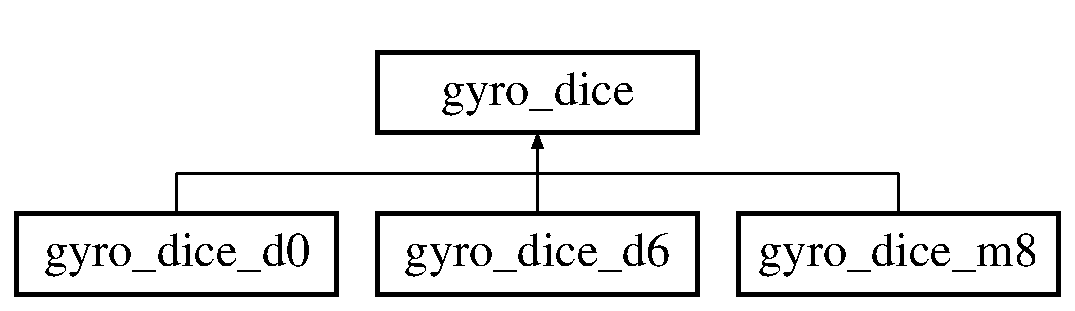
\includegraphics[height=2.000000cm]{classgyro__dice}
\end{center}
\end{figure}
\subsection*{Public Member Functions}
\begin{DoxyCompactItemize}
\item 
\mbox{\Hypertarget{classgyro__dice_a5d9a01ed984a63bdc59a665c75d0059e}\label{classgyro__dice_a5d9a01ed984a63bdc59a665c75d0059e}} 
\hyperlink{classgyro__dice_a5d9a01ed984a63bdc59a665c75d0059e}{gyro\+\_\+dice} (\hyperlink{classgyro__mpu6050}{gyro\+\_\+mpu6050} gyro, hwlib\+::window\+\_\+ostream display, hwlib\+::target\+::pin\+\_\+out beeper)
\begin{DoxyCompactList}\small\item\em \hyperlink{classgyro__dice}{gyro\+\_\+dice} gyrodice constructor, requests a gyroscope, display and a beeper. Updates the dice on initialization. \end{DoxyCompactList}\item 
\mbox{\Hypertarget{classgyro__dice_abdf92bf238356ada218a1bdb560044b1}\label{classgyro__dice_abdf92bf238356ada218a1bdb560044b1}} 
void \hyperlink{classgyro__dice_abdf92bf238356ada218a1bdb560044b1}{update\+\_\+dice} ()
\begin{DoxyCompactList}\small\item\em update\+\_\+dice grabs gyroscope values and works them \end{DoxyCompactList}\item 
\mbox{\Hypertarget{classgyro__dice_ab3bb2c5298f7fb2e53f8b639d4520cf7}\label{classgyro__dice_ab3bb2c5298f7fb2e53f8b639d4520cf7}} 
void \hyperlink{classgyro__dice_ab3bb2c5298f7fb2e53f8b639d4520cf7}{beep\+\_\+dice} ()
\begin{DoxyCompactList}\small\item\em beep\+\_\+dice sends out a beep \end{DoxyCompactList}\item 
\mbox{\Hypertarget{classgyro__dice_a4c3a9c9c4be7988e33ab079278c81f89}\label{classgyro__dice_a4c3a9c9c4be7988e33ab079278c81f89}} 
void \hyperlink{classgyro__dice_a4c3a9c9c4be7988e33ab079278c81f89}{print\+\_\+xyz} ()
\begin{DoxyCompactList}\small\item\em print\+\_\+xyz prints accelX, accelY, accelZ, roll \& pitch variables on the display \end{DoxyCompactList}\item 
\mbox{\Hypertarget{classgyro__dice_afe35725bea57da1a491da5c159fbe201}\label{classgyro__dice_afe35725bea57da1a491da5c159fbe201}} 
void \hyperlink{classgyro__dice_afe35725bea57da1a491da5c159fbe201}{print\+\_\+text} (char str\mbox{[}$\,$\mbox{]})
\begin{DoxyCompactList}\small\item\em print\+\_\+text prints text on the display \end{DoxyCompactList}\item 
\mbox{\Hypertarget{classgyro__dice_a1a6a9e55abb9dad13e516fcd6a6bf7c7}\label{classgyro__dice_a1a6a9e55abb9dad13e516fcd6a6bf7c7}} 
void \hyperlink{classgyro__dice_a1a6a9e55abb9dad13e516fcd6a6bf7c7}{print\+\_\+number} (int i)
\begin{DoxyCompactList}\small\item\em print\+\_\+number prints a number on the display \end{DoxyCompactList}\item 
\mbox{\Hypertarget{classgyro__dice_a6857792a29d9b9ad58ab37e0ccbcf2d3}\label{classgyro__dice_a6857792a29d9b9ad58ab37e0ccbcf2d3}} 
virtual void {\bfseries check\+\_\+side} ()
\item 
\mbox{\Hypertarget{classgyro__dice_a267214c19a7631e8232d9597d9ae1729}\label{classgyro__dice_a267214c19a7631e8232d9597d9ae1729}} 
virtual void {\bfseries set\+\_\+side} ()
\item 
\mbox{\Hypertarget{classgyro__dice_a73b09feb6858574531229a47d3daf84e}\label{classgyro__dice_a73b09feb6858574531229a47d3daf84e}} 
int \hyperlink{classgyro__dice_a73b09feb6858574531229a47d3daf84e}{get\+\_\+acX} ()
\begin{DoxyCompactList}\small\item\em returns acX \end{DoxyCompactList}\item 
\mbox{\Hypertarget{classgyro__dice_aba559b007667feb5887f60881d5bb017}\label{classgyro__dice_aba559b007667feb5887f60881d5bb017}} 
int \hyperlink{classgyro__dice_aba559b007667feb5887f60881d5bb017}{get\+\_\+acY} ()
\begin{DoxyCompactList}\small\item\em returns acY \end{DoxyCompactList}\item 
\mbox{\Hypertarget{classgyro__dice_a8ae424342f37376151625dfd47804db6}\label{classgyro__dice_a8ae424342f37376151625dfd47804db6}} 
int \hyperlink{classgyro__dice_a8ae424342f37376151625dfd47804db6}{get\+\_\+acZ} ()
\begin{DoxyCompactList}\small\item\em returns acZ \end{DoxyCompactList}\end{DoxyCompactItemize}


\subsection{Detailed Description}
\hyperlink{classgyro__dice}{gyro\+\_\+dice}, Default dice simulation 

The documentation for this class was generated from the following files\+:\begin{DoxyCompactItemize}
\item 
\hyperlink{gyro__dice_8hpp}{gyro\+\_\+dice.\+hpp}\item 
gyro\+\_\+dice.\+cpp\end{DoxyCompactItemize}

\hypertarget{classgyro__dice__d0}{}\section{gyro\+\_\+dice\+\_\+d0 Class Reference}
\label{classgyro__dice__d0}\index{gyro\+\_\+dice\+\_\+d0@{gyro\+\_\+dice\+\_\+d0}}


\hyperlink{classgyro__dice__d0}{gyro\+\_\+dice\+\_\+d0}\+:\hyperlink{classgyro__dice}{gyro\+\_\+dice}, random number generator  




{\ttfamily \#include $<$gyro\+\_\+dice.\+hpp$>$}

Inheritance diagram for gyro\+\_\+dice\+\_\+d0\+:\begin{figure}[H]
\begin{center}
\leavevmode
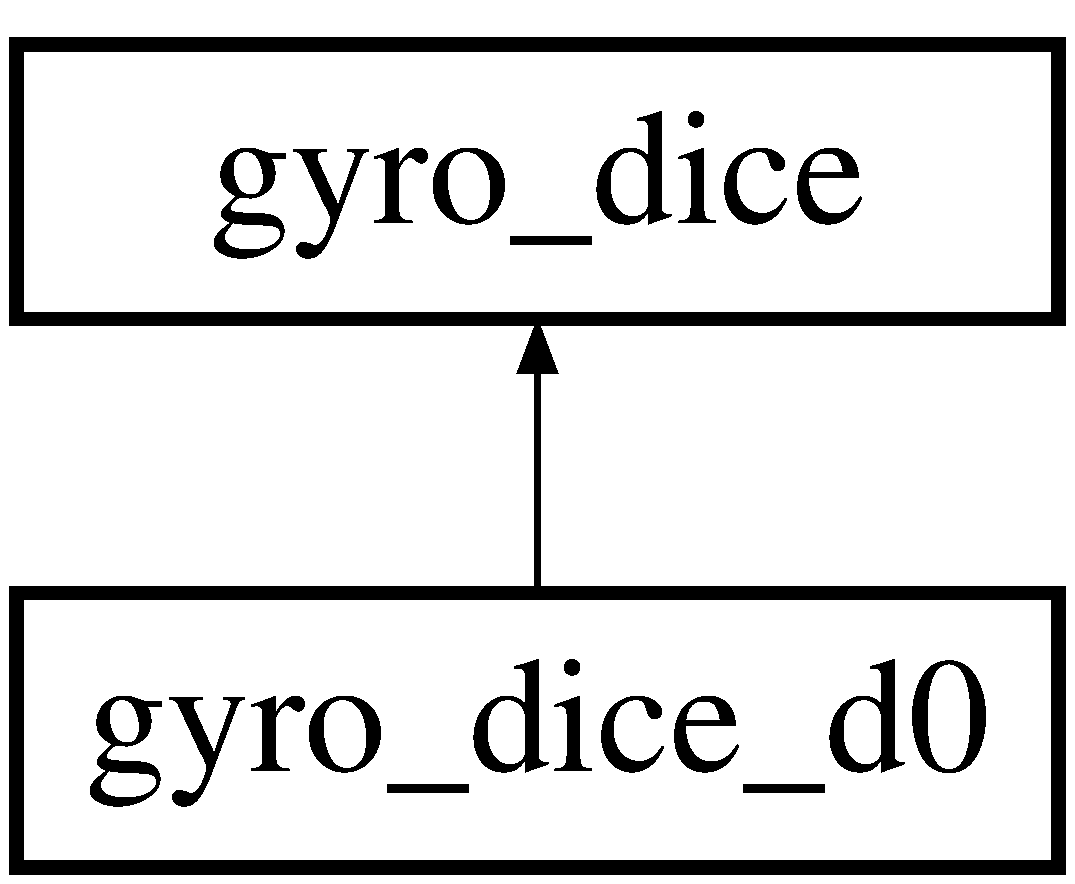
\includegraphics[height=2.000000cm]{classgyro__dice__d0}
\end{center}
\end{figure}
\subsection*{Public Member Functions}
\begin{DoxyCompactItemize}
\item 
\mbox{\Hypertarget{classgyro__dice__d0_a5ff76c0046425a946609726a8896b94c}\label{classgyro__dice__d0_a5ff76c0046425a946609726a8896b94c}} 
\hyperlink{classgyro__dice__d0_a5ff76c0046425a946609726a8896b94c}{gyro\+\_\+dice\+\_\+d0} (\hyperlink{classgyro__mpu6050}{gyro\+\_\+mpu6050} gyro, hwlib\+::window\+\_\+ostream display, hwlib\+::target\+::pin\+\_\+out beeper, int max\+Sides)
\begin{DoxyCompactList}\small\item\em \hyperlink{classgyro__dice__d0}{gyro\+\_\+dice\+\_\+d0} gyrodice d0 constructor, requests a gyroscope, display and a beeper. On initialization starts the internal arduino clock. \end{DoxyCompactList}\item 
\mbox{\Hypertarget{classgyro__dice__d0_ad5b0b46a729eb22c55fada78c2ebec24}\label{classgyro__dice__d0_ad5b0b46a729eb22c55fada78c2ebec24}} 
void \hyperlink{classgyro__dice__d0_ad5b0b46a729eb22c55fada78c2ebec24}{check\+\_\+side} ()
\begin{DoxyCompactList}\small\item\em check\+\_\+side Checks wether a seed has already been generated, if not then generates a seed based on arduino clock. Afterwards checks if the device is being shaken. if it is, prints a random number based on dice sides. \end{DoxyCompactList}\end{DoxyCompactItemize}


\subsection{Detailed Description}
\hyperlink{classgyro__dice__d0}{gyro\+\_\+dice\+\_\+d0}\+:\hyperlink{classgyro__dice}{gyro\+\_\+dice}, random number generator 

The documentation for this class was generated from the following file\+:\begin{DoxyCompactItemize}
\item 
\hyperlink{gyro__dice_8hpp}{gyro\+\_\+dice.\+hpp}\end{DoxyCompactItemize}

\hypertarget{classgyro__dice__d6}{}\section{gyro\+\_\+dice\+\_\+d6 Class Reference}
\label{classgyro__dice__d6}\index{gyro\+\_\+dice\+\_\+d6@{gyro\+\_\+dice\+\_\+d6}}


\hyperlink{classgyro__dice__d6}{gyro\+\_\+dice\+\_\+d6}\+:\hyperlink{classgyro__dice}{gyro\+\_\+dice}, d6 simulation  




{\ttfamily \#include $<$gyro\+\_\+dice.\+hpp$>$}

Inheritance diagram for gyro\+\_\+dice\+\_\+d6\+:\begin{figure}[H]
\begin{center}
\leavevmode
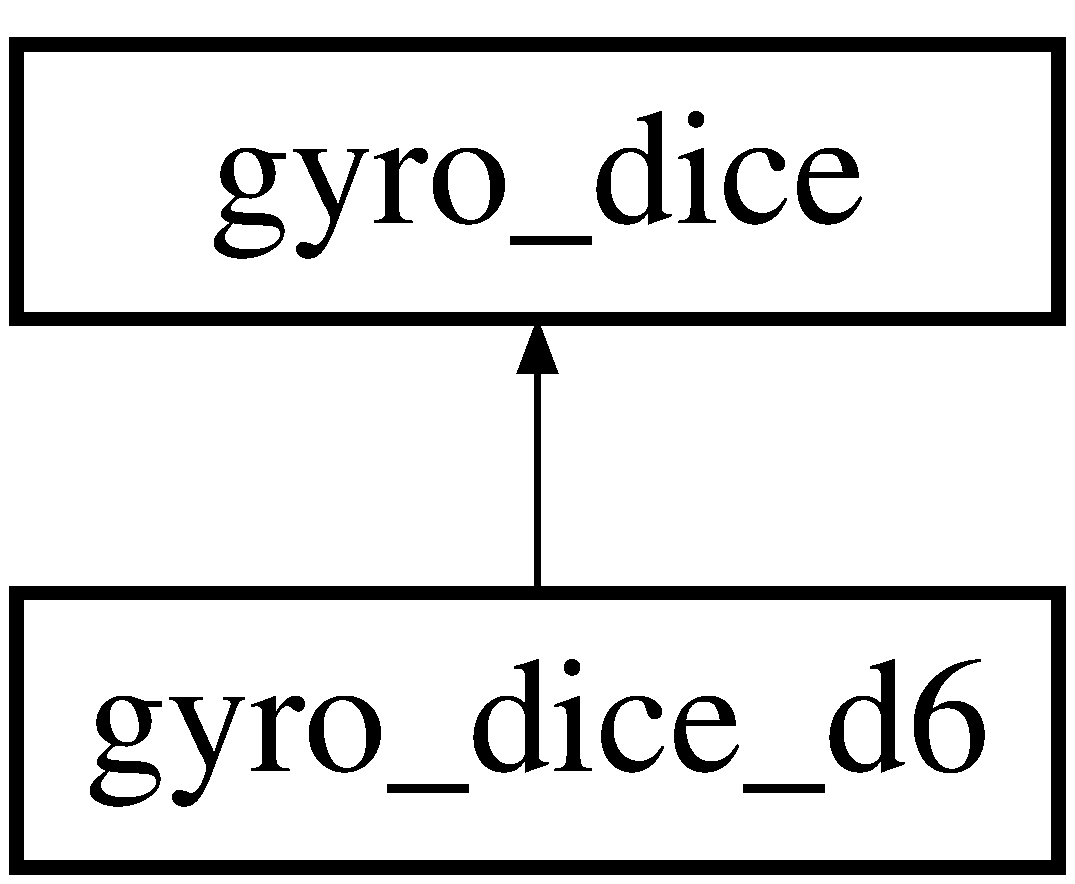
\includegraphics[height=2.000000cm]{classgyro__dice__d6}
\end{center}
\end{figure}
\subsection*{Public Member Functions}
\begin{DoxyCompactItemize}
\item 
\mbox{\Hypertarget{classgyro__dice__d6_ab8c27fd869269f4fdc6fcebc8cadad69}\label{classgyro__dice__d6_ab8c27fd869269f4fdc6fcebc8cadad69}} 
\hyperlink{classgyro__dice__d6_ab8c27fd869269f4fdc6fcebc8cadad69}{gyro\+\_\+dice\+\_\+d6} (\hyperlink{classgyro__mpu6050}{gyro\+\_\+mpu6050} gyro, hwlib\+::window\+\_\+ostream display, hwlib\+::target\+::pin\+\_\+out beeper)
\begin{DoxyCompactList}\small\item\em \hyperlink{classgyro__dice__d6}{gyro\+\_\+dice\+\_\+d6} gyrodice d6 constructor, requests a gyroscope, display and a beeper. \end{DoxyCompactList}\item 
\mbox{\Hypertarget{classgyro__dice__d6_adfed161fb9dec492492bfd54d44e7f20}\label{classgyro__dice__d6_adfed161fb9dec492492bfd54d44e7f20}} 
void \hyperlink{classgyro__dice__d6_adfed161fb9dec492492bfd54d44e7f20}{set\+\_\+side} (int side)
\begin{DoxyCompactList}\small\item\em set\+\_\+side sets the current side of the dice to a new one. \end{DoxyCompactList}\item 
\mbox{\Hypertarget{classgyro__dice__d6_a5efaa5701303b46ec1b9a7bcd451ba25}\label{classgyro__dice__d6_a5efaa5701303b46ec1b9a7bcd451ba25}} 
void \hyperlink{classgyro__dice__d6_a5efaa5701303b46ec1b9a7bcd451ba25}{check\+\_\+side} ()
\begin{DoxyCompactList}\small\item\em check\+\_\+side compares acX, acY and acZ coordinates to the dice sides \end{DoxyCompactList}\item 
\mbox{\Hypertarget{classgyro__dice__d6_a59180a3bc78e6ab0b69867a0d104e789}\label{classgyro__dice__d6_a59180a3bc78e6ab0b69867a0d104e789}} 
void \hyperlink{classgyro__dice__d6_a59180a3bc78e6ab0b69867a0d104e789}{calibrate} ()
\begin{DoxyCompactList}\small\item\em calibrate \mbox{[}N\+YI\mbox{]} dynamically recalibrate the dice \end{DoxyCompactList}\end{DoxyCompactItemize}


\subsection{Detailed Description}
\hyperlink{classgyro__dice__d6}{gyro\+\_\+dice\+\_\+d6}\+:\hyperlink{classgyro__dice}{gyro\+\_\+dice}, d6 simulation 

The documentation for this class was generated from the following file\+:\begin{DoxyCompactItemize}
\item 
\hyperlink{gyro__dice_8hpp}{gyro\+\_\+dice.\+hpp}\end{DoxyCompactItemize}

\hypertarget{classgyro__dice__m8}{}\section{gyro\+\_\+dice\+\_\+m8 Class Reference}
\label{classgyro__dice__m8}\index{gyro\+\_\+dice\+\_\+m8@{gyro\+\_\+dice\+\_\+m8}}


\hyperlink{classgyro__dice__m8}{gyro\+\_\+dice\+\_\+m8}\+:\hyperlink{classgyro__dice}{gyro\+\_\+dice}, magic 8 ball  




{\ttfamily \#include $<$gyro\+\_\+dice.\+hpp$>$}

Inheritance diagram for gyro\+\_\+dice\+\_\+m8\+:\begin{figure}[H]
\begin{center}
\leavevmode
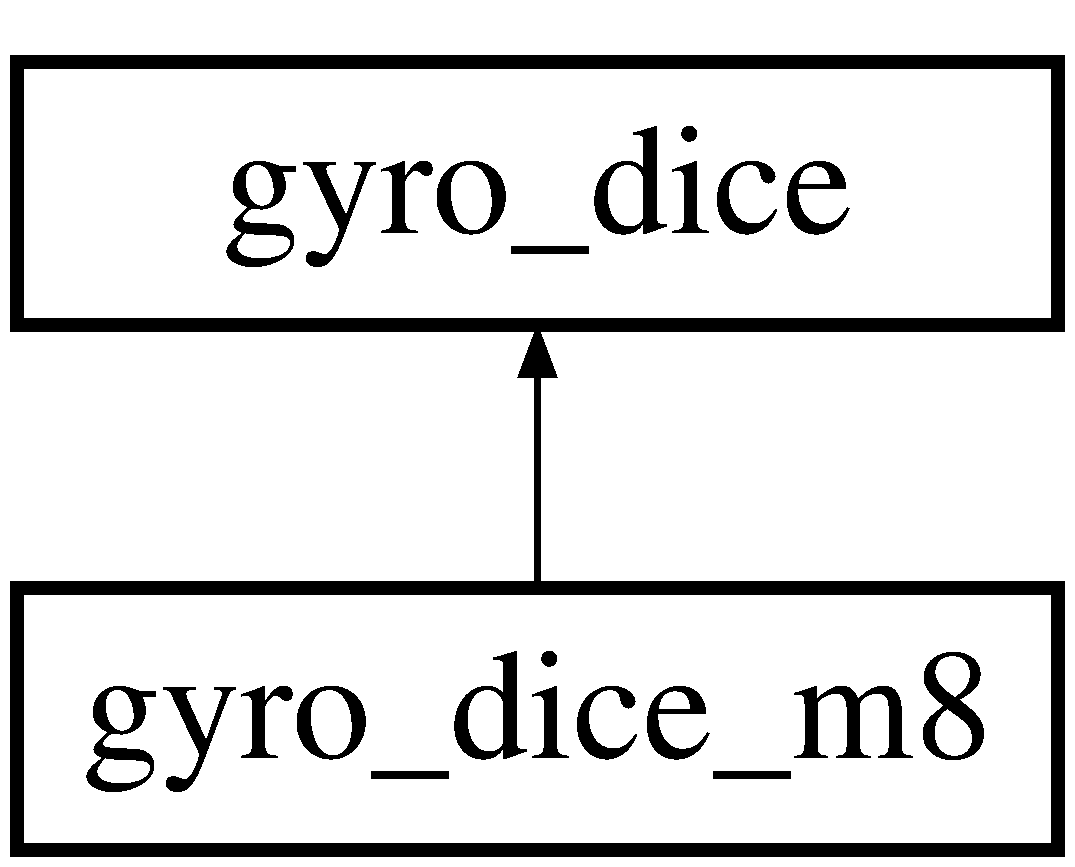
\includegraphics[height=2.000000cm]{classgyro__dice__m8}
\end{center}
\end{figure}
\subsection*{Public Member Functions}
\begin{DoxyCompactItemize}
\item 
\mbox{\Hypertarget{classgyro__dice__m8_ae0f1941a8ba15a6c5ff9be0d012747e2}\label{classgyro__dice__m8_ae0f1941a8ba15a6c5ff9be0d012747e2}} 
\hyperlink{classgyro__dice__m8_ae0f1941a8ba15a6c5ff9be0d012747e2}{gyro\+\_\+dice\+\_\+m8} (\hyperlink{classgyro__mpu6050}{gyro\+\_\+mpu6050} gyro, hwlib\+::window\+\_\+ostream display, hwlib\+::target\+::pin\+\_\+out beeper)
\begin{DoxyCompactList}\small\item\em \hyperlink{classgyro__dice__m8}{gyro\+\_\+dice\+\_\+m8} gyrodice d0 constructor, requests a gyroscope, display and a beeper. On initialization starts the internal arduino clock. \end{DoxyCompactList}\item 
void \hyperlink{classgyro__dice__m8_a1d81aad976c42ef5ac4f8867b0881ad4}{check\+\_\+side} ()
\end{DoxyCompactItemize}


\subsection{Detailed Description}
\hyperlink{classgyro__dice__m8}{gyro\+\_\+dice\+\_\+m8}\+:\hyperlink{classgyro__dice}{gyro\+\_\+dice}, magic 8 ball 

\subsection{Member Function Documentation}
\mbox{\Hypertarget{classgyro__dice__m8_a1d81aad976c42ef5ac4f8867b0881ad4}\label{classgyro__dice__m8_a1d81aad976c42ef5ac4f8867b0881ad4}} 
\index{gyro\+\_\+dice\+\_\+m8@{gyro\+\_\+dice\+\_\+m8}!check\+\_\+side@{check\+\_\+side}}
\index{check\+\_\+side@{check\+\_\+side}!gyro\+\_\+dice\+\_\+m8@{gyro\+\_\+dice\+\_\+m8}}
\subsubsection{\texorpdfstring{check\+\_\+side()}{check\_side()}}
{\footnotesize\ttfamily void gyro\+\_\+dice\+\_\+m8\+::check\+\_\+side (\begin{DoxyParamCaption}{ }\end{DoxyParamCaption})\hspace{0.3cm}{\ttfamily [inline]}, {\ttfamily [virtual]}}

check\+\_\+side Checks wether a seed has already been generated, if not then generates a seed based on arduino clock. Afterwards checks if the device is being shaken. if it is, prints a one of 22 random answers from the answers array.

Reimplemented from \hyperlink{classgyro__dice}{gyro\+\_\+dice}.



The documentation for this class was generated from the following file\+:\begin{DoxyCompactItemize}
\item 
\hyperlink{gyro__dice_8hpp}{gyro\+\_\+dice.\+hpp}\end{DoxyCompactItemize}

\hypertarget{classgyro__mpu6050}{}\section{gyro\+\_\+mpu6050 Class Reference}
\label{classgyro__mpu6050}\index{gyro\+\_\+mpu6050@{gyro\+\_\+mpu6050}}


\hyperlink{classgyro__mpu6050}{gyro\+\_\+mpu6050}, Gyroscope class  




{\ttfamily \#include $<$gyro\+\_\+mpu6050.\+hpp$>$}

\subsection*{Public Member Functions}
\begin{DoxyCompactItemize}
\item 
\mbox{\Hypertarget{classgyro__mpu6050_ab5d528e6eb3d387b5afbd73f911c948f}\label{classgyro__mpu6050_ab5d528e6eb3d387b5afbd73f911c948f}} 
\hyperlink{classgyro__mpu6050_ab5d528e6eb3d387b5afbd73f911c948f}{gyro\+\_\+mpu6050} (hwlib\+::i2c\+\_\+bus\+\_\+bit\+\_\+banged\+\_\+scl\+\_\+sda \&mpu)
\begin{DoxyCompactList}\small\item\em \hyperlink{classgyro__mpu6050}{gyro\+\_\+mpu6050} Gyroscope mpu6050 constructor, requests the i2c bus/adress of the gyroscope. Also wakes up the gyroscope. \end{DoxyCompactList}\item 
\mbox{\Hypertarget{classgyro__mpu6050_a8f2f1da85b970bf7e9f564d80aeef062}\label{classgyro__mpu6050_a8f2f1da85b970bf7e9f564d80aeef062}} 
void \hyperlink{classgyro__mpu6050_a8f2f1da85b970bf7e9f564d80aeef062}{update\+\_\+gyro\+X\+YZ} (uint16\+\_\+t \&x, uint16\+\_\+t \&y, uint16\+\_\+t \&z)
\begin{DoxyCompactList}\small\item\em update\+\_\+gyro\+X\+YZ Obtains raw gyroscope data from the mpu6050 each axis exists of 2 bytes, a high and a low byte, then mashes them together \end{DoxyCompactList}\item 
\mbox{\Hypertarget{classgyro__mpu6050_a8700adda96c44677ae97c53f9bf9808d}\label{classgyro__mpu6050_a8700adda96c44677ae97c53f9bf9808d}} 
void \hyperlink{classgyro__mpu6050_a8700adda96c44677ae97c53f9bf9808d}{update\+\_\+accel\+X\+YZ} (uint16\+\_\+t \&x, uint16\+\_\+t \&y, uint16\+\_\+t \&z)
\begin{DoxyCompactList}\small\item\em update\+\_\+accel\+X\+YZ Obtains raw accelerometer data from the mpu6050 \end{DoxyCompactList}\item 
\mbox{\Hypertarget{classgyro__mpu6050_a5b41f980fa2a0a944e8cf9794f7d4c70}\label{classgyro__mpu6050_a5b41f980fa2a0a944e8cf9794f7d4c70}} 
void \hyperlink{classgyro__mpu6050_a5b41f980fa2a0a944e8cf9794f7d4c70}{update\+\_\+temp} (uint16\+\_\+t \&tmp)
\begin{DoxyCompactList}\small\item\em update\+\_\+temperature Obtains raw temperature data from the mpu6050 \end{DoxyCompactList}\item 
\mbox{\Hypertarget{classgyro__mpu6050_a1462eef299ea464162b2113d9a14928d}\label{classgyro__mpu6050_a1462eef299ea464162b2113d9a14928d}} 
void \hyperlink{classgyro__mpu6050_a1462eef299ea464162b2113d9a14928d}{update\+\_\+all} ()
\begin{DoxyCompactList}\small\item\em update\+\_\+all Updates all data of the gyroscope \end{DoxyCompactList}\item 
\mbox{\Hypertarget{classgyro__mpu6050_a99f8993b2e3af57de308a7162317bb59}\label{classgyro__mpu6050_a99f8993b2e3af57de308a7162317bb59}} 
uint16\+\_\+t \hyperlink{classgyro__mpu6050_a99f8993b2e3af57de308a7162317bb59}{get\+\_\+tmp} ()
\begin{DoxyCompactList}\small\item\em returns gyroscope tmp \end{DoxyCompactList}\item 
\mbox{\Hypertarget{classgyro__mpu6050_acc6e1e14ee53040db09c37bf439f7506}\label{classgyro__mpu6050_acc6e1e14ee53040db09c37bf439f7506}} 
uint16\+\_\+t \hyperlink{classgyro__mpu6050_acc6e1e14ee53040db09c37bf439f7506}{get\+\_\+gyroX} ()
\begin{DoxyCompactList}\small\item\em returns gyroscope X \end{DoxyCompactList}\item 
\mbox{\Hypertarget{classgyro__mpu6050_a56f90145147ca6f7afeef6870a4abaf1}\label{classgyro__mpu6050_a56f90145147ca6f7afeef6870a4abaf1}} 
uint16\+\_\+t \hyperlink{classgyro__mpu6050_a56f90145147ca6f7afeef6870a4abaf1}{get\+\_\+gyroY} ()
\begin{DoxyCompactList}\small\item\em returns gyroscope Y \end{DoxyCompactList}\item 
\mbox{\Hypertarget{classgyro__mpu6050_a955e5fc73fb60db70d9fd21d9845041c}\label{classgyro__mpu6050_a955e5fc73fb60db70d9fd21d9845041c}} 
uint16\+\_\+t \hyperlink{classgyro__mpu6050_a955e5fc73fb60db70d9fd21d9845041c}{get\+\_\+gyroZ} ()
\begin{DoxyCompactList}\small\item\em returns gyroscope Z \end{DoxyCompactList}\item 
\mbox{\Hypertarget{classgyro__mpu6050_ac121cf3b8dcc2655585a17c587ed7250}\label{classgyro__mpu6050_ac121cf3b8dcc2655585a17c587ed7250}} 
uint16\+\_\+t \hyperlink{classgyro__mpu6050_ac121cf3b8dcc2655585a17c587ed7250}{get\+\_\+accelX} ()
\begin{DoxyCompactList}\small\item\em returns accelerometer x \end{DoxyCompactList}\item 
\mbox{\Hypertarget{classgyro__mpu6050_ab0ab2bbd7875ccad4c244b6496764f35}\label{classgyro__mpu6050_ab0ab2bbd7875ccad4c244b6496764f35}} 
uint16\+\_\+t \hyperlink{classgyro__mpu6050_ab0ab2bbd7875ccad4c244b6496764f35}{get\+\_\+accelY} ()
\begin{DoxyCompactList}\small\item\em returns accelerometer y \end{DoxyCompactList}\item 
\mbox{\Hypertarget{classgyro__mpu6050_af90c1ec0103b8c7b168f32779302b96e}\label{classgyro__mpu6050_af90c1ec0103b8c7b168f32779302b96e}} 
uint16\+\_\+t \hyperlink{classgyro__mpu6050_af90c1ec0103b8c7b168f32779302b96e}{get\+\_\+accelZ} ()
\begin{DoxyCompactList}\small\item\em returns accelerometer z \end{DoxyCompactList}\end{DoxyCompactItemize}


\subsection{Detailed Description}
\hyperlink{classgyro__mpu6050}{gyro\+\_\+mpu6050}, Gyroscope class 

The documentation for this class was generated from the following file\+:\begin{DoxyCompactItemize}
\item 
\hyperlink{gyro__mpu6050_8hpp}{gyro\+\_\+mpu6050.\+hpp}\end{DoxyCompactItemize}

\chapter{File Documentation}
\hypertarget{gyro__dice_8hpp}{}\section{gyro\+\_\+dice.\+hpp File Reference}
\label{gyro__dice_8hpp}\index{gyro\+\_\+dice.\+hpp@{gyro\+\_\+dice.\+hpp}}
\subsection*{Classes}
\begin{DoxyCompactItemize}
\item 
class \hyperlink{classgyro__dice}{gyro\+\_\+dice}
\begin{DoxyCompactList}\small\item\em \hyperlink{classgyro__dice}{gyro\+\_\+dice}, Default dice simulation \end{DoxyCompactList}\item 
class \hyperlink{classgyro__dice__d6}{gyro\+\_\+dice\+\_\+d6}
\begin{DoxyCompactList}\small\item\em \hyperlink{classgyro__dice__d6}{gyro\+\_\+dice\+\_\+d6}\+:\hyperlink{classgyro__dice}{gyro\+\_\+dice}, d6 simulation \end{DoxyCompactList}\item 
class \hyperlink{classgyro__dice__d0}{gyro\+\_\+dice\+\_\+d0}
\begin{DoxyCompactList}\small\item\em \hyperlink{classgyro__dice__d0}{gyro\+\_\+dice\+\_\+d0}\+:\hyperlink{classgyro__dice}{gyro\+\_\+dice}, random number generator \end{DoxyCompactList}\item 
class \hyperlink{classgyro__dice__m8}{gyro\+\_\+dice\+\_\+m8}
\begin{DoxyCompactList}\small\item\em \hyperlink{classgyro__dice__m8}{gyro\+\_\+dice\+\_\+m8}\+:\hyperlink{classgyro__dice}{gyro\+\_\+dice}, magic 8 ball \end{DoxyCompactList}\end{DoxyCompactItemize}
\subsection*{Macros}
\begin{DoxyCompactItemize}
\item 
\mbox{\Hypertarget{gyro__dice_8hpp_aa63d0ef44bde54f6e9b3b74ca4e20af4}\label{gyro__dice_8hpp_aa63d0ef44bde54f6e9b3b74ca4e20af4}} 
\#define {\bfseries degconvert}~57.\+2957786
\item 
\mbox{\Hypertarget{gyro__dice_8hpp_af736091baab3dac91dc7a8412008368d}\label{gyro__dice_8hpp_af736091baab3dac91dc7a8412008368d}} 
\#define {\bfseries display\+\_\+width}~128
\item 
\mbox{\Hypertarget{gyro__dice_8hpp_a235fb0c5a01a7aa25bac6d3284b873e3}\label{gyro__dice_8hpp_a235fb0c5a01a7aa25bac6d3284b873e3}} 
\#define {\bfseries display\+\_\+height}~64
\end{DoxyCompactItemize}

\hypertarget{gyro__mpu6050_8hpp}{}\section{gyro\+\_\+mpu6050.\+hpp File Reference}
\label{gyro__mpu6050_8hpp}\index{gyro\+\_\+mpu6050.\+hpp@{gyro\+\_\+mpu6050.\+hpp}}
\subsection*{Classes}
\begin{DoxyCompactItemize}
\item 
class \hyperlink{classgyro__mpu6050}{gyro\+\_\+mpu6050}
\begin{DoxyCompactList}\small\item\em \hyperlink{classgyro__mpu6050}{gyro\+\_\+mpu6050}, Gyroscope class \end{DoxyCompactList}\end{DoxyCompactItemize}

\hypertarget{main_8cpp}{}\section{main.\+cpp File Reference}
\label{main_8cpp}\index{main.\+cpp@{main.\+cpp}}
{\ttfamily \#include \char`\"{}hwlib.\+hpp\char`\"{}}\newline
{\ttfamily \#include \char`\"{}gyro\+\_\+mpu6050.\+hpp\char`\"{}}\newline
{\ttfamily \#include $<$cmath$>$}\newline
{\ttfamily \#include \char`\"{}gyro\+\_\+dice.\+hpp\char`\"{}}\newline
\subsection*{Functions}
\begin{DoxyCompactItemize}
\item 
\mbox{\Hypertarget{main_8cpp_a840291bc02cba5474a4cb46a9b9566fe}\label{main_8cpp_a840291bc02cba5474a4cb46a9b9566fe}} 
int \hyperlink{main_8cpp_a840291bc02cba5474a4cb46a9b9566fe}{main} (void)
\begin{DoxyCompactList}\small\item\em main Sets up the oled and gyroscope mpu6050 which then afterwards are used to simulate the dice. \end{DoxyCompactList}\end{DoxyCompactItemize}

%--- End generated contents ---

% Index
\backmatter
\newpage
\phantomsection
\clearemptydoublepage
\addcontentsline{toc}{chapter}{Index}
\printindex

\end{document}
